\documentclass[PICOAPC.tex]{subfiles}

\begin{document}

PICO will produce 21 polarization maps of Galactic emission, all much deeper than \planck 's seven maps. At 799~GHz PICO will have five times finer resolution than \planck . %; see Fig.~\ref{fig:allsky}). 
Such a dataset can only be obtained by a space mission like PICO. These data will complement a rich array of other polarization observations forthcoming in the next decade, including stellar polarization surveys to be combined with \gaia~astrometry, and Faraday rotation measurements from  observations at radio wavelengths with the  Square Kilometer Array and its precursors. \\
%
% \begin{figure}[h]
% \vspace{-0.22in}
%\hspace{0.2in}
%\parbox{2.7in}{\centerline {
%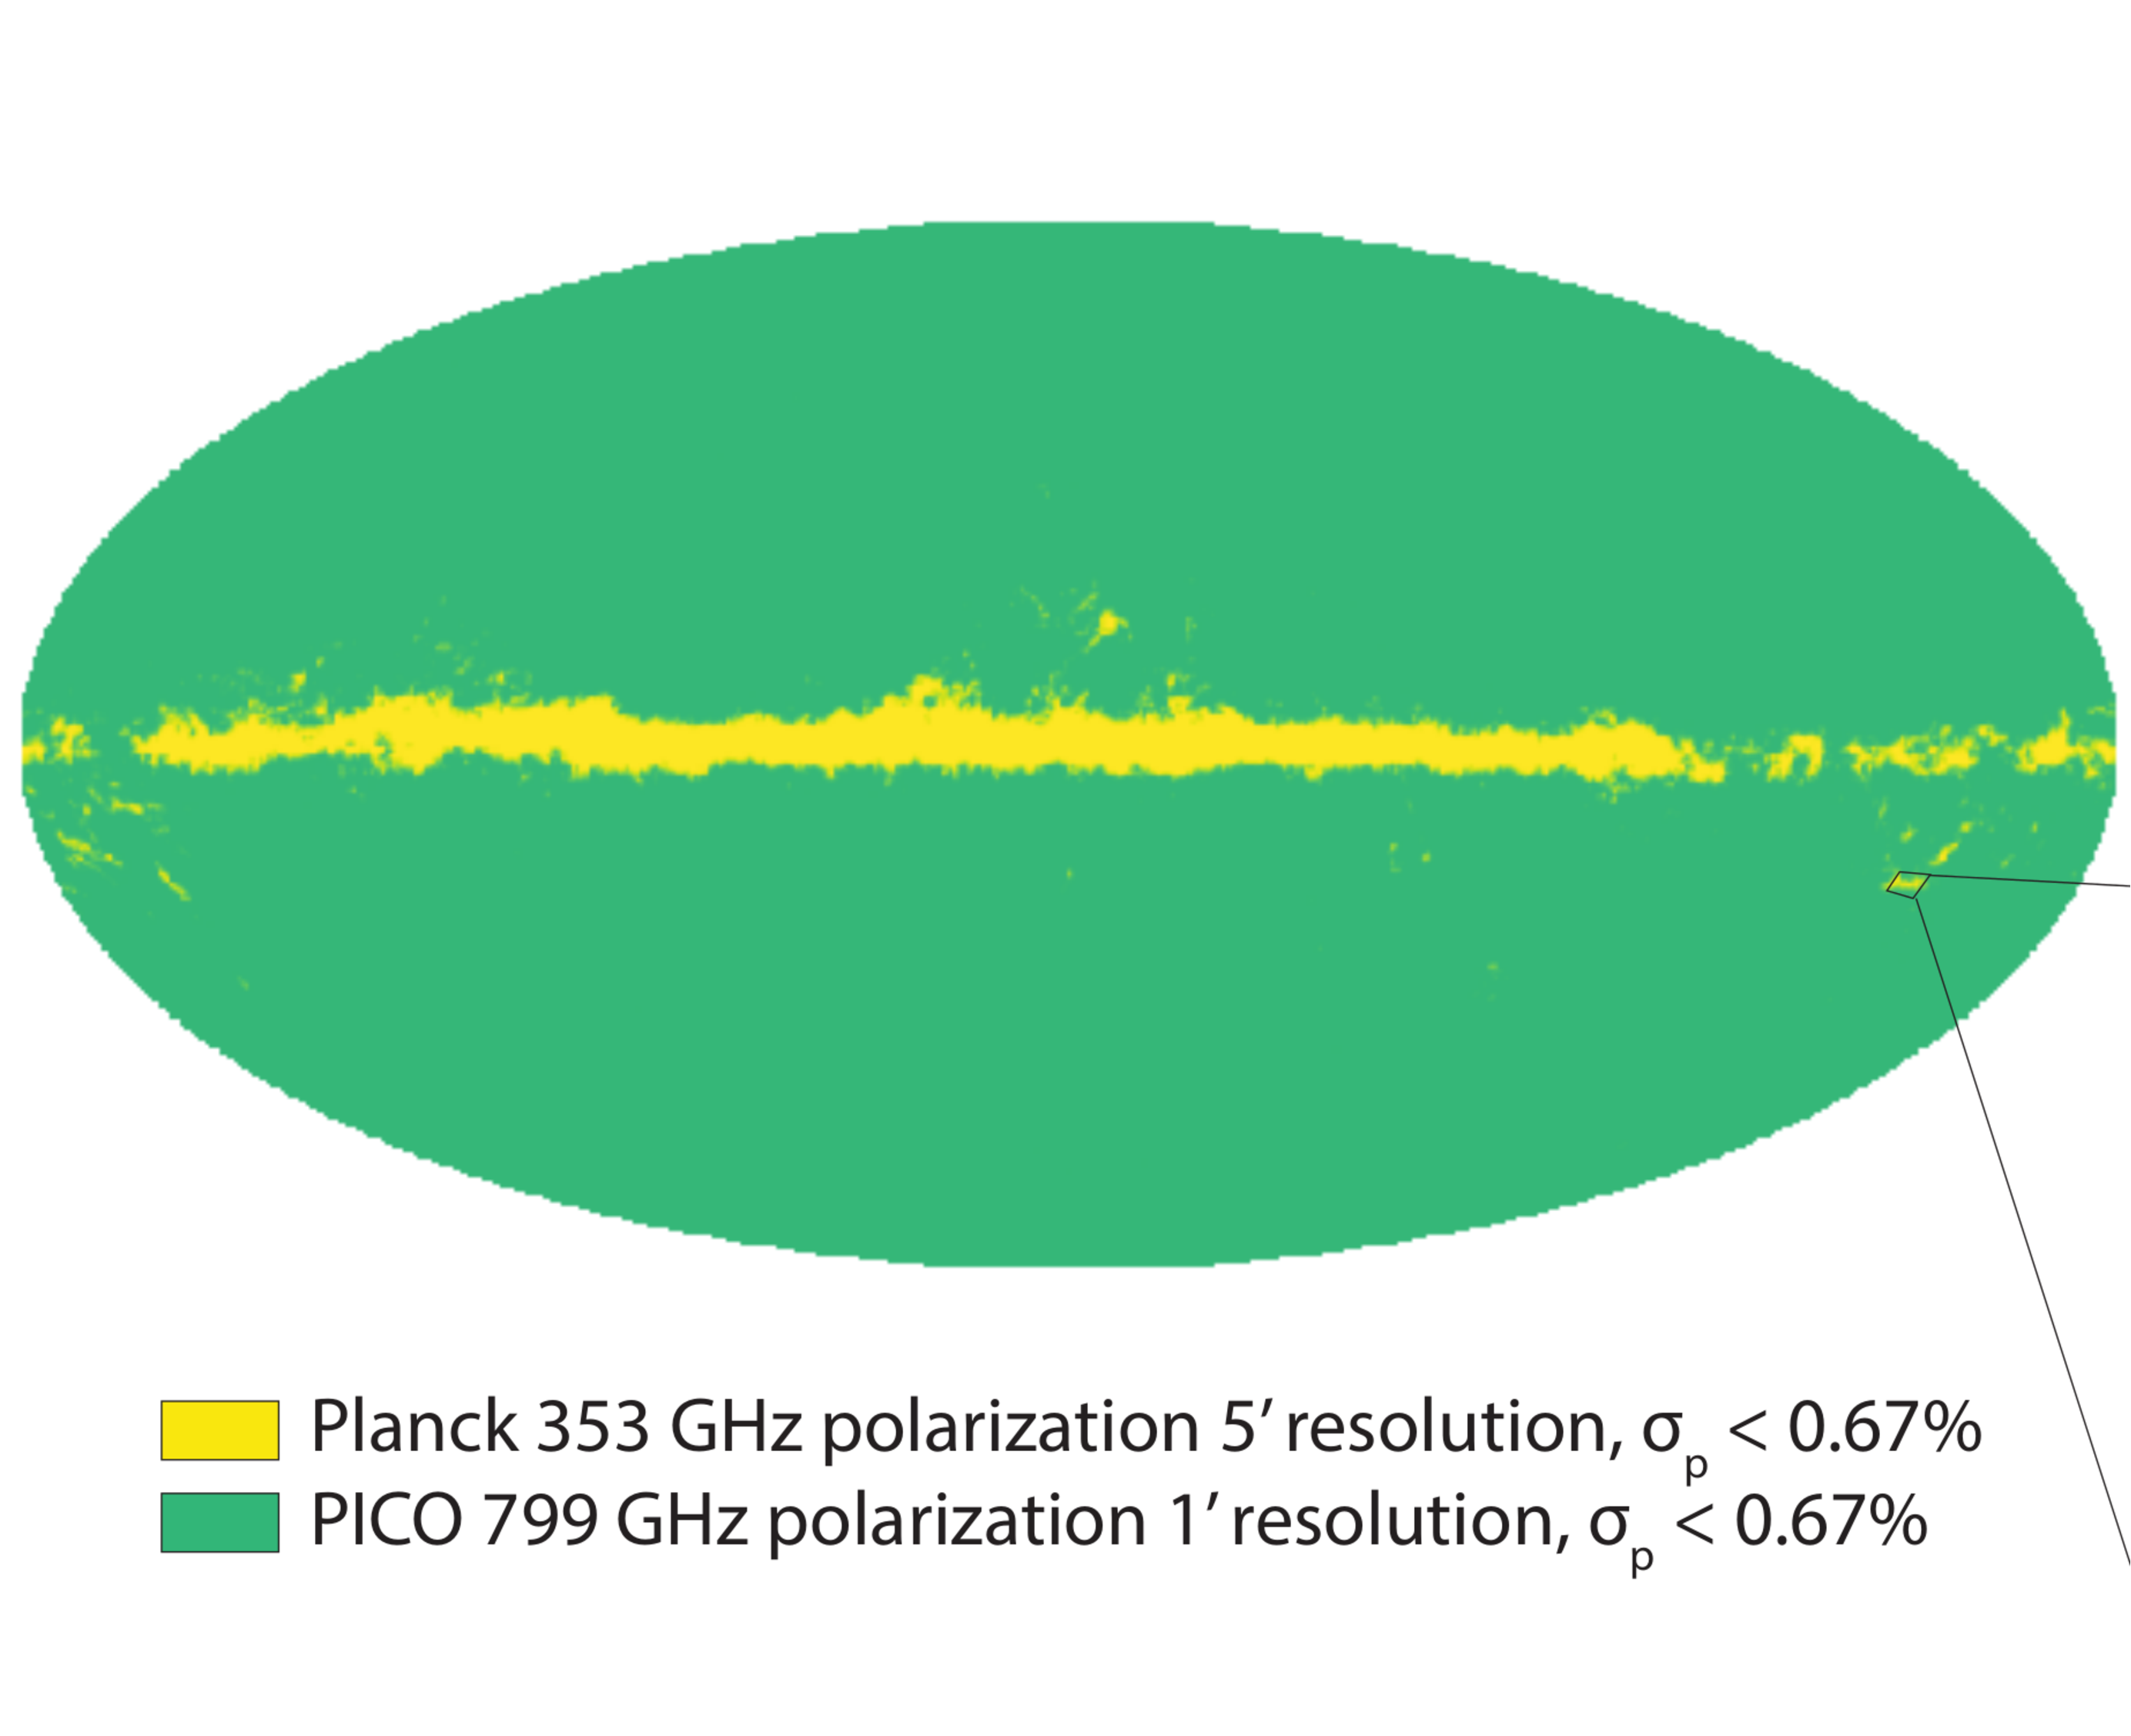
\includegraphics[width=2.5in]{galsci_fig_v4_cropped.pdf} } }
%\hspace{0.in}
%\parbox{3.8in}{
%\caption{\captiontext Caption will be here
%%    \caption{\captiontext  \planck 's 353~GHz polarization map gave a resolution of 5\arcmin~and sensitivity to polarization intensity of $\sigma_{p} < 0.67\%$ over a small portion of the sky (left, yellow).  At 799 GHz, the PICO baseline mission will give a polarization map of the {\it entire sky} and with 5 times higher resolution (left, green). In the middle panels, the \planck~map of the Orion region overlaid with vectors that are aligned with the inferred magnetic field (lower panel), and a simulated PICO observation (upper panel) illustrate the leap in information content (vector lengths are proportional to polarization fraction). With this map, and maps at other frequencies, PICO will characterize Galactic magnetized turbulence at scales spanning the diffuse ISM down to dense star-forming cores, which will be mapped with high-resolution polarimetry by instruments such as HAWC+/SOFIA~\citep{Chuss2018} (right panel) and ALMA~\citep{Bacciotti2018ApJ}. }
%\label{fig:fom} } }
%\vspace{-0.13in}
%\end{figure}
%
% \begin{figure}[h]
% \vspace{0.1in}
%\hspace{0.6in}
%\parbox{2.7in}{\centerline {
%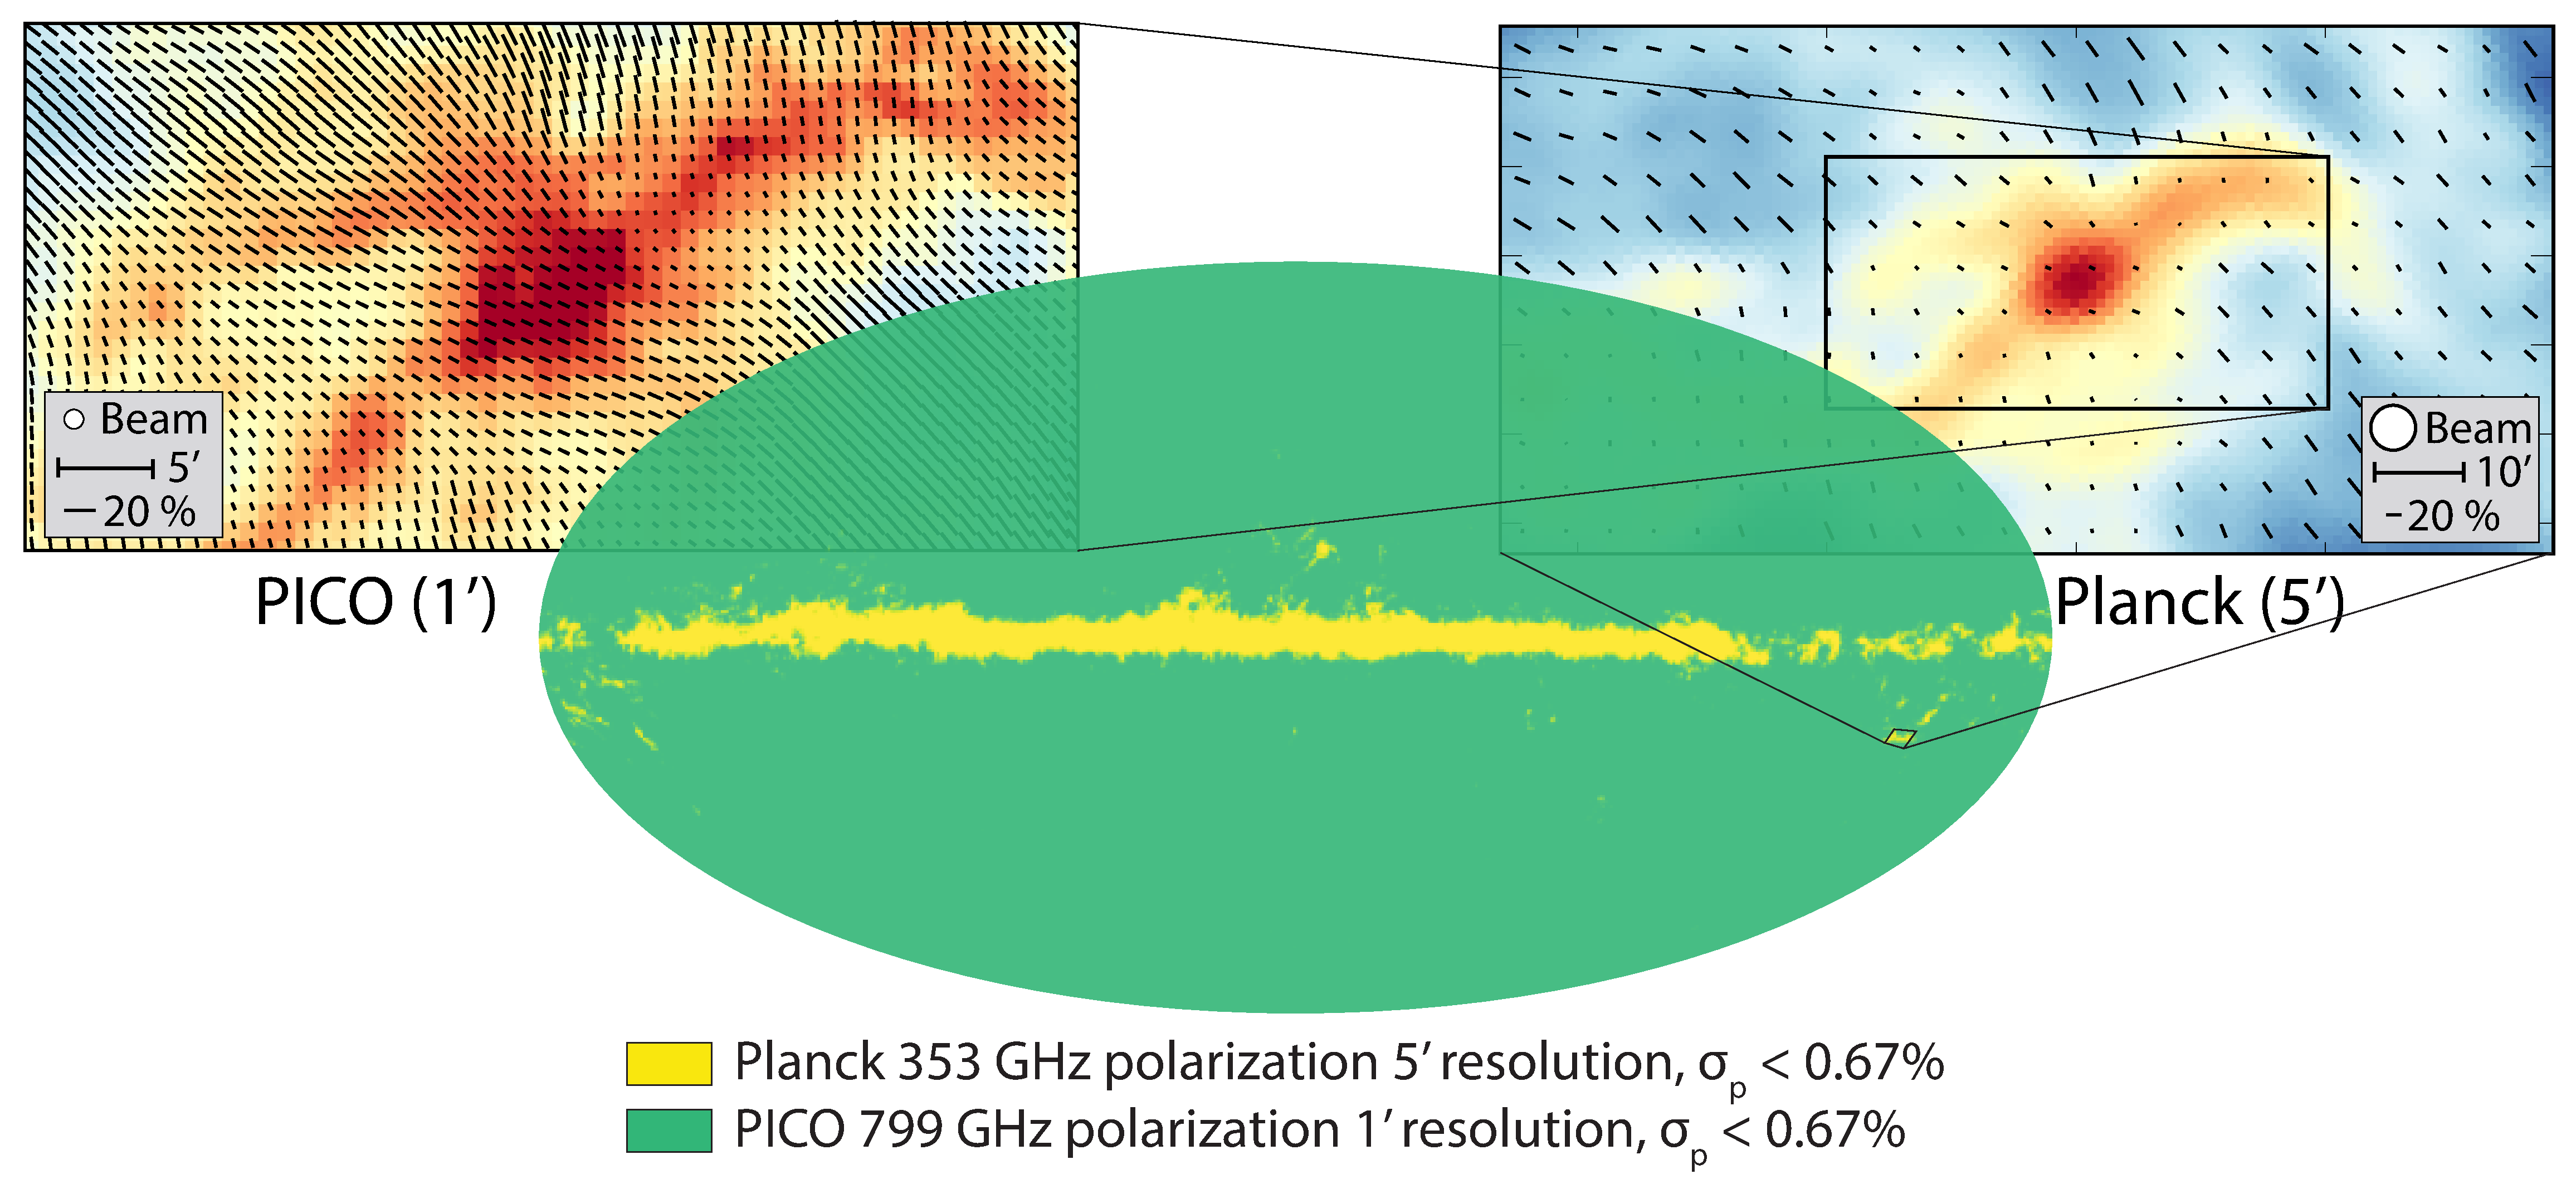
\includegraphics[width=4.0in]{galsci_fig_v5.pdf} } }
%%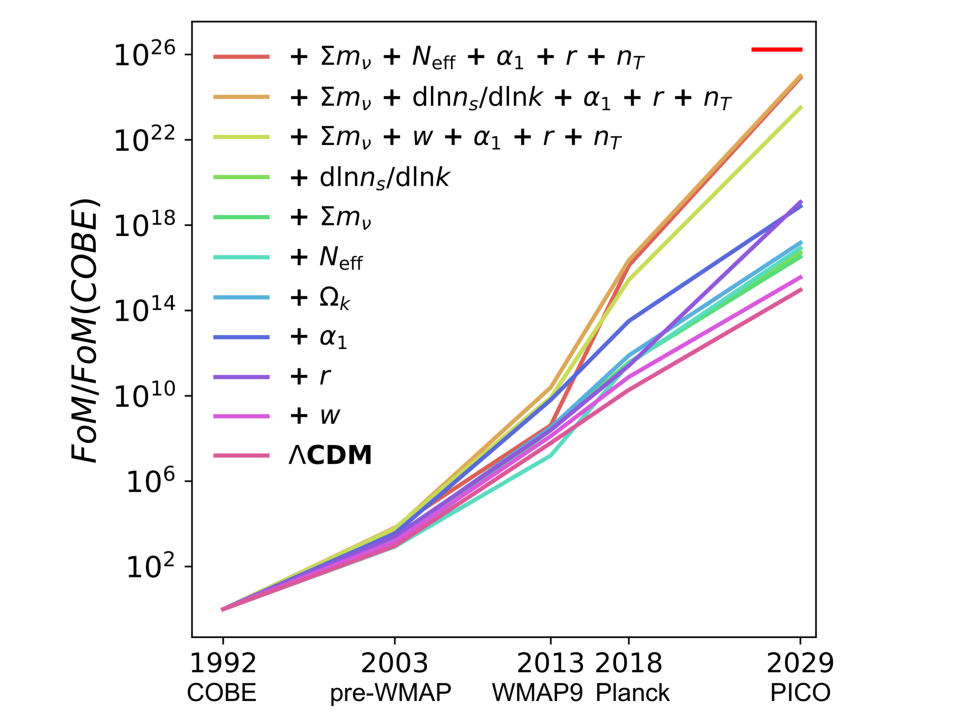
\includegraphics[width=3.0in]{images/fom_plot_CVL+del.pdf} } }
%\hspace{0.in}
%\parbox{3.8in}{
%\caption{\captiontext Caption will be here
%%    \caption{\captiontext  \planck 's 353~GHz polarization map gave a resolution of 5\arcmin~and sensitivity to polarization intensity of $\sigma_{p} < 0.67\%$ over a small portion of the sky (left, yellow).  At 799 GHz, the PICO baseline mission will give a polarization map of the {\it entire sky} and with 5 times higher resolution (left, green). In the middle panels, the \planck~map of the Orion region overlaid with vectors that are aligned with the inferred magnetic field (lower panel), and a simulated PICO observation (upper panel) illustrate the leap in information content (vector lengths are proportional to polarization fraction). With this map, and maps at other frequencies, PICO will characterize Galactic magnetized turbulence at scales spanning the diffuse ISM down to dense star-forming cores, which will be mapped with high-resolution polarimetry by instruments such as HAWC+/SOFIA~\citep{Chuss2018} (right panel) and ALMA~\citep{Bacciotti2018ApJ}. }
%\label{fig:fom} } }
%\vspace{-0.13in}
%\end{figure}
%
%While the PICO maps will likely provide new insights and surprises, we focus here on two particularly important science objectives: (1) Test models of the composition of interstellar dust, and (2) Determine how magnetic fields affect molecular cloud and star formation. \\
$\bullet$ {\bf Test Models of the Composition of Interstellar Dust} \hspace{0.1in}  
Less than a few $\mu$m in size, dust grains are intermediate in the evolution from atoms and molecules to large solid bodies such as comets, asteroids, and planets. Through vastly improved spectral characterization of Galactic polarization, the PICO data will 
%discriminate among models of Galactic dust composition to elucidate the chemical evolution of the Galaxy. For example, for the two-component paradigm \citep{Meisner2015}, the PICO baseline mission will determine the intrinsic polarization fractions of each of the two components to a precision of 3\%. With this level of precision the data will 
validate or reject state-of-the-art dust models~\citep[e.g.][]{Draine2009,Guillet2018,hensely_swp}, test for the presence of additional dust grain species with distinct polarization signatures, such as magnetic nanoparticles~\citep{Draine2013}, and will be used as an input for the foreground separation necessary to extract cosmological $E$- and $B$-mode science. \\
$\bullet$ {\bf Determine How Magnetic Fields Affect Molecular Cloud and Star Formation} \hspace{0.1in}
Stars are formed through interactions between gravitational and magnetic fields, turbulence, and gas over more than four orders of magnitude of spatial scales, which span the diffuse ISM (kpc scale), molecular clouds (10~pc), and molecular cloud cores (0.1~pc). However, the role magnetic fields play in the large-scale structure of the diffuse interstellar medium and in the observed low star-formation efficiency has been elusive, owing to the dearth of data. 
With 1.1~arcmin resolution PICO will expand the number of independent magnetic field measurements across the sky from \planck 's  30,000 to 86,000,000, a factor of 2900. The data will robustly characterize turbulent properties like the Alfv\'{e}n Mach number across a previously unexplored regime of parameter space. 
%With full-sky coverage, PICO will map all the molecular clouds out to a distance of 3.4\,kpc with better than 1\,pc resolution; we estimate there will be over 2,000 clouds that will be mapped with $10^3$--$10^5$  independent polarization measurements per cloud. These are the {\it only foreseeable} measurements that will give the ratio of the energies stored in magnetic and gravitational fields, and the ratio of the energy stored in the magnetic field to that stored in gas turbulence over a statistically significant sample of molecular clouds.

\end{document}

%\begin{figure}[!htb]
%\centering
%\includegraphics[width=4cm]{images/example}
%\caption{example}
%\label{fig:im_3}
%\end{figure}
